\documentclass[oneside,b5paper,11pt]{article} %book class in 11 points
\usepackage{geometry} % Package re-sizing page for b5paper
\usepackage[hangul]{kotex} % Korean support
\usepackage{natbib} % cite style
\usepackage{paralist} % package for inline enumerate, i) ii)...

\usepackage{graphicx} % Allows including images

\usepackage{amsmath} % for math symbols
\usepackage{amssymb} % for math symbols

\usepackage{tablefootnote} % to use table foot note

%\graphicspath{ {D:/_PlayGround/Github/2016_thesis/tex/images} }
\graphicspath{ {C:/My/Playground/Git/2016_Thesis/tex/images/} }

\kscntformat{section}{}{} % 제 1.1절 -> 1.1
\renewcommand\thesection{\arabic{section}.} % 제 1.1절 -> 1.1
\renewcommand\thesubsection{\indent\arabic{section}.\arabic{subsection}.}


%%들여쓰기
\usepackage{indentfirst}
\setlength\parindent{2.0em}


\title{Ideas scattered}
\author{김동완}
\date{\today}

\begin{document}

%%%%%%%%%%
% Starting document.
%%%%%%%%%%


%\maketitle



% Section
\section{서론}
\subsection{What to say?}
지금, 요즘 시대의 데이터에 기존의 방법론을 사용하는 것에 어떤 문제가 있는가? 왜 그런 문제가 생기는 것인가? 요즘 데이터의 특징이 무엇이길레 이런 문제가 생기는 것인가? 기존의 방법론은 어떤 특성을 갖고 있는가?

\subsection{Online learning and batch learning}
Most existing learning to rank techniques follow batch and offline machine learning methodology, which typically assumes all training data are available prior to the learning task and the ranking model is trained by applying some batch learning method.

One of serious limitations perhaps is its poor scalability for real-world web applications, where the ranking model has to be re-trained from scratch whenever new training data arrives. This is apparently inefficient and non-scalable since training data often arrives sequentially and frequently in many real applications [33, 7]. Besides, batch learning to rank methodology also suffers from slow adaption to fast-changing environment of web applications due to the static ranking models pre-trained from historical batch training data.

a new framework of Scalable Online Learning Algorithms for Ranking, which aims to learn a ranking model from a sequence of training data in an online learning fashion.

\subsection{요즘 데이터가 어떠한가? C​haracteristics of big data?}
http://www.dummies.com/how-to/content/characteristics-of-big-data-analysis.html




\subsection{blabla}
 우리는 데이터 폭증의 시대에 살고 있다. 웹 로그, IoT기기 로그, 게임 로그 등 단일 서비스에서 하루에 발생하는 로그의 양은 상상을 초월한다. 예를들어 facebook의 하루 로그 크기는 600TB정도\footnote{https://code.facebook.com/posts/229861827208629/scaling-the-facebook-data-warehouse-to-300-pb/}로서 기존의 통계 분석 방법으로는 간단한 인사이트 조차 얻기 어려운 경우가 많다. 그리고 데이터의 규모가 커진 것 뿐만 아니라 급변하는 사용자 요구 사항과 경쟁자의 출현에 맞서 거의 실시간으로 이러한 데이터를 분석해 빠른 의사결정을 하거나 즉각적인 서비스를 제공하는 등의 대응을 해야하는 상황에 직면하고 있다. 또한 데이터의 건수가 많아지는 문제와 더불어 다수의 범주형 변수와 각 범주형 변수마다 수백 수천개의 범주가 있고 시간이 지남에 따라 예측할 수 없는 다양한 범주가 추가될 수 있는 형태의 데이터를 분석해야 하는 경우도 생겨난다.

 예를들어 TrueSkill과 같이 다량의 플레이어 게임 메칭 데이터를 이용해 플레이어의 승률을 계산하여 최적의 게임 메칭 상태를 찾는 문제\citep{Herbrich2006}, 특정 Facebook 사용자의 timeline에 다양한 조건의 광고 중 어떤 광고를 노출 시켜야 광고 클릭 확률이 높을 것인지를 예측하는 문제\citep{He2014}, 매출의 대부분을 차지하는 고부가 가치 유저(High-Valued Player)가 게임에서 이탈할 확률을 계산하는 문제\citep{Runge2014} 등은 대규모 데이터 분석과 빠른 예측이 비즈니스의 성패를 좌우하는 경우라고 할 수 있다. 이러한 문제를 풀기 위해서는 규모 가변적이고 대규모의 분산 데이터 처리\footnote{Scalable Massive Distributed Data Processing}를 위한 하드웨어와 소프트웨어, 그리고 이에 맞는 분석 방법론이 필요하고 본 논문에서는 분석 방법론에 대해 고찰해 볼 것이다.
 
 앞서의 상황과 같이 유동적 다변량의 다샘플 데이터를 실시간으로 분석하는 것은 기존 배치방식의 통계 분석으로는 효과적이지 않다. 가령 데이터가 스트리밍으로 유입되고 이를 분석 데이터에 추가하고 모수 값을 계산해야하는 상황에서 매번 전체 데이터에 대해 모형 적합을 수행해서는 실시간에 가까운 예측 결과를 내놓기 어렵다. 또한 새로운 변수 혹은 범주가 데이터 세트에 추가될 때마다 모수 벡터를 다시 구성하고 모형 적합을 다시 수행하는 것은 좋은 접근법이라 할 수 없다. 

본 논문에서는 배치 방식에 대비되는 온라인 모형 적합 방법을 샘플 수가 수천만건에 이르고 다수의 범주형 변수, 그리고 범주의 개수가 유동적인 대규모 데이터에 적용하기 위한 모형 적합 방법과 해싱을 이용한 가변수 코딩(Feature Hashing)에 대해 고려해 보고 각 방법의 특성에 대해서 고찰해 볼 것이다. 또한 가상 데이터와 실제 데이터에에 각 방법론의 적용해 보고 각각의 특성을 실증적으로 살펴볼 것이다. 이를 위해 2장 1절에서는 최적화 알고리즘의 하나인 경사하강법(Gradient Descent)과 확률적 경사하강법(Stochastic Gradient Descent)에 대해 알아보고, 2장 2절에서는 이항 반응 변수에 가장 일반적으로 적용 가능한 로지스틱 회귀 모형과 이에 대한 베이지안 접근 방법에 대해 알아볼 것이다. 또한 2장 3절에서는 확률적 경사하강법의 베이지안 접근 방법이라 할 수 있는 추정된 밀도 필터링(Assumed-Density Filtering) 방법에 대해서 알아볼 것이다. 3장에서는 앞서 소개한 방법론에 대한 실증적 분석으로서 먼저 3장 1절 에서는 가상 데이터를 생성하여 SGD와 ADF 방법을 적용해 볼 것이다. 그리고 3장 2절에서 소규모 이항반응 데이터에 두 방법을 적용해 볼 것이며 3장 3절에서는 대규모 이방반응 데이터를 포함하는 사례 데이터에 대한 분석을 통해서 SGD와 ADF에 대한 비교 분석을 실시한다. 마지막으로 4장에서는 본 논문의 결론과 향구 과제를 논의한다.



% Section
\section{Feature Hashing}
\subsection{What to say?}
 언제? 왜 사용하는가? 또한 어떤 기법들이 있고, 각각의 장단점은 무엇인가? 그중에서 어떤 것을 왜 사용할 것인가?
\subsection{Answers}
Refer to [http://blog.reverberate.org/2012/01/state-of-hash-functions-2012.html]

Why?
 다수의 변수가 포함되어 있거나 범주형 변수의 범주가 많은 자료를 분석하고자 하는 경우 차원을 축소(Dimensionality reduction)하고 가변수 값의 성김(sparsity)으로 인한 많은 메모리 사용량 문제를 해결하고, 빠르게 데이터 레코드에 해당하는 메모리 상의 feature 벡터의 값에 접근하게 하고, 온라인 학습에서는 매 분석 시점마다 범주형 변수의 범주가 추가될 수도 있는 문제를 해결하기 위해 Feature Hashing을 사용한다.

What kinds of?
 해싱 방식은 크게 암호방식과 비암호방식으로 나뉜다. 암호방식은 해싱 성능 보다는 해시값 복호화가 어려워야 한다는 중요한 특성을 갖도록 고안된 방식이다. 반면 비암호화 방식은 복호과가 가능하느냐는 중요하지 않고 해싱을 수행하는 속도와 해시 결과의 분포적 특성에 중점을 둔 방식이다. 여기서 분포적 특성이란 입력값이 문자열 상으로 유사하더라도 그 결과는 어느 구간에 밀집되지 않고 전체 해시 공간에 고르게 분포하는 것을 말한다.\citep{Ramadhian2013} 속도 측면에서는 대표적인 암호화 해시 방식인 SHA-1이 0.09 bytes/cycle의 해싱 속도를 갖는 반면 비암호화 해시의 하나인 MurmurHash의 경우 1 byte/cycle의 속도로서 거의 10배 가량 빠르다. 

 물론 Feature hashing을 사용하는 것이 장점만이 있는 것은 아니다. 대표적인 문제로 해시 충돌을 들 수 있다. 분포도가 양호한 해시 방식을 사용하는 것이 가장 우선 이겠으나 해시 충돌은 발생할 수 있는 문제이고, 이를 줄이기 위해 해시 함수에 입력될 문자열을 모든 변수의 범주를 통틀어 가능한 유일 하도록 매핑하는 작업을 하거나 피쳐 벡터(feature vector)의 크기를 고려하여 해시 테이블 크기를 조정 하는 것도 한 방법이다.













\section{SGD, Stochastic Gradient Descent / 확률적 경사 하강법}
\subsection{What to say?}
SGD는 무엇이고 언제 사용하는가? 어떤 특성을 갖고 있는가? 단점은 없는가? 단점에 대한 대안은 없는가?

\subsection{Answers}
https://www.quora.com/Whats-the-difference-between-gradient-descent-and-stochastic-gradient-descent
http://leon.bottou.org/publications/pdf/compstat-2010.pdf


최적화(optimization) 알고리즘의 하나인 경사하강법(Gradient descent)에서는 전체 샘플 데이터를 스캔 할 때마다 회귀 계수 추정치를 갱신해 나간다. 비용함수(cost function)을 $J(w) = \frac{1}{2} \sum_{i}(target^{(i)} - output^{(i)})^{2}$ 라 할때 매 갱신($w_{i+1}=w_{i}+\Delta w$)에서 $j$개의 모수 추정치($w$)를 얼마만큼 줄일지 혹은 늘릴지 $\Delta w$ 값을 결정해야 한다. 여기에서 $\Delta w$는 아래와 같다.
\begin{eqnarray}
\Delta w_{j} 	&=& -\alpha \frac{\delta J}{\delta w_{j}} \\
							&=& -\alpha \sum_{i}(target^{(i)} - output^{(i)})(-x^{(i)_{j}}) \\
							&=& \alpha \sum_{i}(target^{(i)} - output^{(i)})(x^{(i)_{j}})
\end{eqnarray}
즉 비용함수(cost function)의 경사도가 크면 그만큼 많이 $w$값을 수정하게 되는데, 학습 계수(learning rate, step size) $\alpha$에 비례하여 수정치가 결정된다.

 경사하강법에서는 한번 $w$값을 수정하기 위하여 전체 샘플 데이터를 스캔하게 된다. 그런데 이런 방식은 샘플의 수가 많은 경우 
비용함수 $J(w)$를 최소로 하는 $w$값을 찾기 까지 그 처리 시간이 길어 지게 된다. 모수에 대한 학습(learning)이나 추론(inference)를 진행할 때 데이터의 크기가 작거나 데이터의 수집으로부터 예측까지 시간적 여유가 있을 경우 데이터 전체를 한꺼번에 활용하는 일괄 처리(batch processing) 방식을 사용한다. 반면 데이터를 한꺼번에 처리하기에 그 크기가 지나치게 크거나 스트리밍(streaming)으로 유입되는 데이터에 대해서 실시간으로 예측을 처리해야 하는 경우 온라인 학습(online learning)을 사용해야 할 필요성이 있다.

 이처럼 매 갱신에서 전체 샘플 데이터를 사용하는 대신 샘플 하나 혹은 일부분만을 사용하여 $w$ 값을 갱신해 가는 방법을 확률적 경사 하강법(Stochastic Gradient Descent, Online Gradient Descent)이라 하며, 확률적 이라는 단어에서 알 수 있듯이 $J(w)$를 최소로 하는 $w$의 참값을 확률적 근사 값을 찾아가는 방법이다. 하나의 샘플만을 이용해 $w$의 갱신 방향과 크기를 결정하기 때문에 경사하강법과는 달리 $J(w)$값이 커지는 경우도 있으나 샘플 수가 충분할 경우 $J(w)$의 전역 최소값으로 수렴하는 $w$를 찾을 수 있는 것으로 알려져 있다. \citep{Bottou2010}

 경사 하강법 혹은 확률적 경사 하강법의 성능을 결정하는 가장 중요한 요소는 학습 계수(learning rate) $\alpha$인데, 모형이 근사적으로 수렴하기 위해서는 이 값을 점차 줄여나가야만 한다. $\alpha$ 값을 줄여 나가는 방법으로는 반복(iteration)의 진행횟수에 비례하여 $\alpha_{t+1} = \alpha_{t} / (1 + t \times d )$와 같이 $\alpha$ 값을 감소 시키는 방법이나, 알고리즘의 성능에 따라 $\alpha$값을 변화시키는 방법 등이 있다. 

 회귀 모형과 같이 선형 가우시안을 가정하는 경우 이 문제를 \citet{Kalman1960}의 칼만 필터(Kalman filter)와 같이 접근할 수도 있다. 온라인 학습에서 가장 가까운 미래 시점의 모수 값 혹은 분포를 추정하는 것을 흔히 필터링(filtering)이라 하고, 과거 시점의 그것을 추정하는 것을 스무딩(smoothing)이라 한다. 온라인 필터링 알고리즘으로는 칼만 필터\citep{Kalman1960}, 칼만 필터의 비선형 버전이라 할 수 있는 확장 칼만 필터\citep{Smith1962}, 무향 변환(unscented transform)을 이용한 가우시안 근사로 확장 칼만 필터를 개선한 무향 칼만 필터\citep{Julier1997}, 사전 분포와 측정값을 이용하여 적률 대응(moment matching)으로 사후 분포를 근사하는 추정된 밀도 필터(Assumed Density Filtering)\citep{Opper1996} 등이 있다.
 
 추정된 밀도 필터(Assumed Density Filtering)은 베이지안 접근 방법으로서 \citet{Opper1996}가 제안한바 있는데, 매 반복마다 하나의 샘플을 이용하여 $w$값을 갱신하는데 있어서 $t$ 시점에서 $w$의 분포를 생각하고 이때 사용할 하나의 샘플을 이용하여 사후 분포를 구한다. 다시 $t+1$ 시점에서는 이전 시점에서의 사후 분포를 사전분포로 활용하여 계속하여 $w$의 분포를 갱신해 나가는 것이다. 이러한 접근 방법에서는 $w$의 불확실성을 해당 분포의 분산의 크기로 모형화한 것이라 할 수 있다. 



\section{논문에서 하려는 예기는 무엇인가?}
\subsection{What to say?}
 본 논문에서는 이러한 기존의 연구결과들(\citet{Bottou2010}; \citet{Opper1996}을 샘플 수가 수천만건에 이르고 다수의 범주형 변수, 그리고 범주의 개수가 유동적인 대규모 데이터에 적용하기 위한 방법을 고려해 보고 각 방법의 특성에 대해서 고찰해 볼 것이다. 또한 가상 데이터와 실제 데이터에에 각 방법론의 적용해 보고 각각의 특성을 실증적으로 살펴볼 것이다. 이를 위해 먼저 ()절 에서는 가상 데이터를 생성하여 SGD와 ADF 방법을 적용해 볼 것이다. 그리고 () 절에서 소규모 이항반응 데이터에 두 방법을 적용해 볼 것이다. 마지막으로 ()절에서는 사례연구(대규모 이방반응 데이터)를 통해서 SGD와 ADF에 대한 실증적 비교 분석을 실시한다. 마지막으로 ()절에서는 본 논문의 결론과 향구 과제를 논의한다.


\section{시뮬레이션}
\subsection{What to say?}
3가지 시뮬레이션, 
1. 가상 데이터를 이용한 단순선형회귀
2. 타이타닉 데이터(범주형 데이터)
3. 광고 데이터
이런 시뮬레이션이 준비 되어 있긴한데, 어떤 수치를 통해서 결과를 제시해야 할지 모르겠다. 두 방법론을 비교한다는데, 어떤 지표를 이용해서 비교해야할지 모르겠다. 꼭 비교를 해야하는가? 아니면 대용량, 다변수 데이터를 분석하는 방법을 알아보는 것으로 가면 안 될까? 어떤 대상과 비교해서 성능의 우위를 갖는 방법론을 제시할만한 깜량이 못 된다.

 1번 시뮬레이션이 그토록 구려서 쓰기 그렇다면, 2번부터 적어보자. 


\subsection{타이타닉 데이터..}
성능 평가 기준.. 다양한 metric 값들, ROC curve
https://www.kaggle.com/wiki/LogarithmicLoss


\subsection{타이타닉 데이터..}
 타이타닉 탑승자들의 여러 특성에 따른 생존 여부를 나타내는 889건의 데이터\footnote{https://www.kaggle.com/c/titanic/data}에 대한 분석을 진행해 보았다. 데이터는 생존여부를 나타내는 이항 반응변수와 승객의 10가지 특성을 나타내는 설명변수로 구성되어 있다. 데이터에서 대체로 유의미하지 않은 정보를 갖고 있는 승객의 이름, 티켓번호와 결측치가 77$\%$에 이르는 객실 번호는 분석에서 제외하고, 나이 값의 20$\%$ 정도 결측치는 평균치로 대체하였다. 전체 데이터 중 800건을 훈련 자료(training data) 나머지 89건을 테스트 자료(test data)로 구분하여 사용하였다.
 우선 훈련 자료를 이용하여 생존여부를 반응변수로 하는 로지스틱 회귀 모형에 대하여 '배치 방식의 최대 가능도 추정', '확률적 경사 하강법', '추정된 밀도 필터링'을 각각 적용하여 예측 성능을 비교해 보기로 한다. 예측 성능에 대한 지표를 살펴 보았다.


\begin{table}[ht]
	\centering
	\begin{tabular}{cccccccccc}
	\hline\hline
	%\toprule
	\textbf{} & \textbf{TP} & \textbf{FP} & \textbf{FN} & \textbf{TN} & \textbf{Accu} & \textbf{Prec} & \textbf{Recall} & \textbf{F1-Score} & \textbf{logloss}  \\ 
	\hline 
	%\midrule
	
	\multicolumn {1}{l|}{MLE} & 24 & 9  & 5 & 41 & 0.843 & 0.727 & 0.826 & 0.774 & 37.679 \\ \hline
	\multicolumn {1}{l|}{SGD} & 22 & 11 & 6 & 50 & 0.809 & 0.667 & 0.786 & 0.721 & 36.608 \\ \hline
	\multicolumn {1}{l|}{ADF} & 21 & 12 & 7 & 49 & 0.787 & 0.636 & 0.750 & 0.688 & 38.859 \\ \hline

	\hline
	%\bottomrule
	\end{tabular}
	
	\caption[예측률 비교]{예측률 비교\tablefootnote{$logloss = -\frac{1}{N}\sum_{i=1}^N {(y_i\log(p_i) + (1 - y_i)\log(1 - p_i))}$}}
\end{table}



\begin{center}
\includegraphics[scale=0.55]{titanic_roc.eps} %730 * 430
\end{center}


\section{맺음말}
\subsection{What to say?}
 이런 방법과 저런 방법을 이런 데이터에 적용해 보았다. 이런 데이터의 특성상 피쳐 해싱을 사용해야 했고, 이럴 경우 이러한 장점을 얻었다.
베이지안 접근 방법에 있어서 Gibbs sampling 방법을 이용한 접근은 표본 추출 시간 때문에 대용량 데이터에 대한 온라인 러닝 상황을 해결하기 어렵다. 베이지안 접근 방법이 필요할 경우 이와 같은 근사 분포를 사용하는 방법론이 효과적이다. 
또한 구현상에서는 R과 Pthon을 통해 모두 구현해 보았는데 절대적으로 Python을 이용한 구현이 실행속도 면에서 압도적이었다. 4500만건 트레이닝 상황에서 R을 이용한 구현에서는 대략 2주정도 실행 시간이 예상되었으나 Python을 이용한 구현에서는 불과 2시간만에 결과를 얻을 수 있었다. 물론 구현 방식과 사용하는 패키지에 따라서 차이가 있겠으나 실시간 실행 시간이 중요한 상황에서는 R을 통한 구현에는 한계가 있어 보인다. 
SGD의 경우 alpha의 초기값에 그리고 ADF의 경우 모수들의 초기 분산 값에 모형 적합 결과가 아주 크게 좌우 되었다.
또한 다수의 가변적인 범주를 포함하는 다변수 데이터에 대한 온라인 러닝에서 필수적이라 할 수 있는 feature hashing에 대해서 고려해 보았다.

1. 이런 저런거 해 봤다.
2. Feature hashing
2. 베이지안 접근 방법 구현에 있어서 고려점
3. 구현에 잇어서 유의점
4. SGD, ADF의 성능에 영향을 주는 요소



\subsection{Here we go}
 본 논문에서는 다변수 대용량 데이터에 대한 실시간 모형 적합 방법과 구현시 고려 사항에 대해 고려해 고찰해 보았다. 우선 데이터의 규모가 커질 경우 배치 방식의 한계점으로 인하여 온라인 방식의 모형 적합 방법을 적용해야 했고, 대표적인 온라인 모형 적합 방법인 확률적 경사 하강법(Stochastic Gradient Descent)과 이 방법의 베이지안 접근이라 할 수 있는 추정된 밀도 필터링(Assumed-Density Filtering) 방법을 사용하여 예측 결과의 추이를 살펴보았다. 

일반적으로 베이지안 접근 방법은 대규모 데이터 처리에 적합하지 않다는 주장이 많다. 하지만 Gibbs Sampling이 아니라 추정된 밀도 필터링과 같은 근사 분포를 사용하는 방법론을 사용할 경우 실시간 처리가 필수적인 온라인 러닝에 있어서도 충분히 만족스러운 속도로 분석을 진행 할 수 있음을 확인 할 수 있었다. 또한 컴퓨팅 속도를 향상 시킬 수 있는 프로그래밍 언어, GPU 컴퓨팅, 분산 처리 기법등을 적용할 경우 방법론 선택에 대한 제약은 크지 않다고 할 수 있다.

실제로 동일한 알고리즘을 R과 Pthon을 통해 모두 구현해 보았는데 절대적으로 Python을 이용한 구현이 실행속도 면에서 압도적이었다. 4500만건 트레이닝 상황에서 R을 이용한 구현에서는 대략 2주정도 실행 시간이 예상되었으나 Python을 이용한 구현에서는 불과 2시간만에 결과를 얻을 수 있었다. 물론 구현 방식과 사용하는 패키지에 따라서 차이가 있겠으나 빠른 실행 시간이 필요한 상황에서는 어떤 프로그래밍 언어를 선택하느냐가 중요한 요소일 수 있다.

모수 벡터 설정 및 변수 코딩과 관련하여 다범주 다변수 데이터를 실시간 분석해야할 경우 해싱을 이용한 접근 방법을 사용하는 것이 효과적임을 확인할 수 있었다. 우선 단순히 차원 축소 뿐만 아니라 각 셈플 벡터의 크기가 줄어 메모리 사용량이 줄어들고 모수 벡터에 대한 빠른 접근이 가능하여 실행 성능 향상 효과를 얻을 수 있었고 대략적인 변수 규모만 지정하면 범주가 추가될 경우에도 다시 가변수 코딩이나 적합을 수행할 필요가 없는 장점을 확인 할 수 있었다.

 확률적 경사 하강법의 경우 '스텝 크기' $\alpha$를 어떻게 조절 하느냐가 예측 결과에 아주 큰 영향을 주었다. $\alpha$를 반복횟수에 반비례하여 조절할 경우 우수한 예측 결과를 얻을 수 있었으나 $\alpha$의 초기값에 따라 모형의 성능이 크게 좌우 되었다. 반면 추정된 밀도 필터링의 경우 각 모수 분포의 분산($\sigma$) 초기값에 따라 모형의 성능이 변할 수 있음을 확인 할 수 있었다. 또한 $\sigma$값에 따라 확률적 경사하강법에 비해 초기에 낮은 log-loss값을 보여주기도 했으나, 적합 반복이 증가할 경우 두 모형 사이에 절대적인 우위를 확인할 수는 없았다. 결국 확률적 경사 하강법에서는 '스텝 크기' $\alpha$, 추정된 밀도 필터링에서는 각 모수 분포의 분산($\sigma$) 초기값을 적절히 설정하느냐가 모형의 성능을 결정하는 중요한 요소임을 알 수 있었다.


%
% Reference
%
\bibliographystyle{apalike}
\bibliography{thesis_dwKim_references}

\end{document}